\documentclass{standalone}
\usepackage{pgfplots}
\pgfplotsset{compat=1.17}

\begin{document}

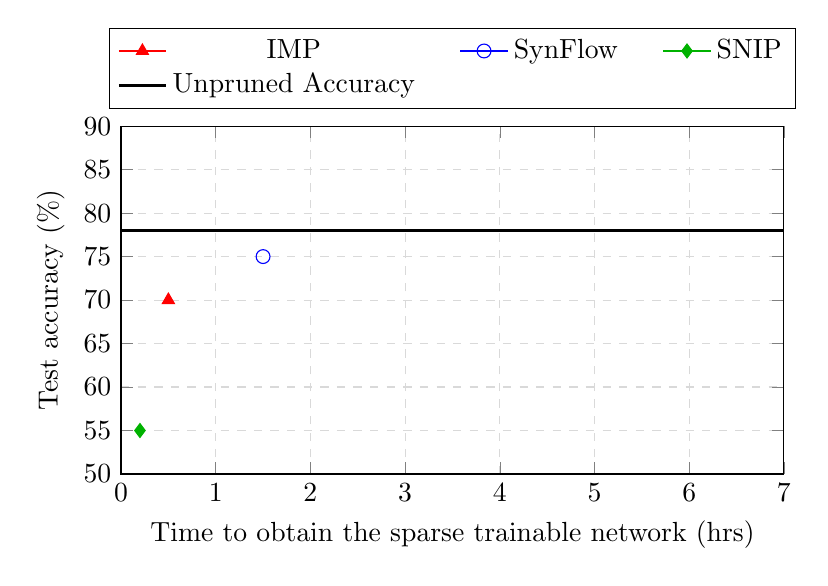
\begin{tikzpicture}
\begin{axis}[
    width=10cm, height=6cm,
    xlabel={Time to obtain the sparse trainable network (hrs)},
    ylabel={Test accuracy (\%)},
    ymin=50, ymax=90,
    xmin=0, xmax=7,
    xtick={0, 1, 2, 3, 4, 5, 6, 7},
    ytick={50, 55, 60, 65, 70, 75, 80, 85, 90},
    grid=both,
    grid style={dashed, gray!30},
    legend style={at={(0.5,1.05)}, anchor=south, legend columns=3, /tikz/every even column/.append style={column sep=0.5cm}}
]

\addplot[red, mark=triangle*, mark size=2.5pt] coordinates {
    (0.5, 70)
};
\addlegendentry{IMP}

\addplot[blue, mark=o, mark size=2.5pt] coordinates {
    (1.5, 75)
};
\addlegendentry{SynFlow}

\addplot[green!70!black, mark=diamond*, mark size=2.5pt] coordinates {
    (0.2, 55)
};
\addlegendentry{SNIP}

\addplot[black, thick] coordinates {
    (0, 78) (7, 78)
};
\addlegendentry{Unpruned Accuracy}

\end{axis}
\end{tikzpicture}

\end{document}